
\documentclass{beamer}

\usepackage[T1]{fontenc}
\usepackage[utf8]{inputenc}
\usepackage[english]{babel}
\usepackage{multirow}
\usepackage{lmodern}
\usepackage{multicol}
\usepackage{default}
\usepackage[list=true]{subcaption}
\captionsetup{compatibility=false}
\usecolortheme{cormorant}
\useoutertheme{infolines}


\title[GnuPG]{H4ck 1n TN}
\subtitle{GnuPG}
\author[H4ck1nTN]{Gabrielle \textsc{toulet morlanne}\\%
Olivier \textsc{dautricourt}\\%
Benoît \textsc{tallandier}}
\institute[HiT]{Ceten -- TELECOM Nancy}
\date{20 octobre 2016}
\logo{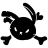
\includegraphics[width=1.3cm]{figures/logo_black.png}}

\setbeamercolor{section in toc}{fg=black}
\setbeamercolor{subsection in toc}{fg=darkgray}
\begin{document}


\begin{frame}
\titlepage
\end{frame} 

% BODY %

\begin{frame}{Plan}
	\tableofcontents[
currentsubsection, 
sectionstyle=show, 
subsectionstyle=show, 
] 
\end{frame}

\begin{frame}{Prérequis}

\begin{itemize}
\item Paquets nécessaires : gnupg2, thunderbird, enigmail. \\
\item Installation : \\
\textbf{sudo apt-get install gnupg2 thunderbird enigmail} (debian, mint, \\
		\hspace*{0.8cm}	|\textbf{yum} (Fedora) \hspace*{5.4cm} ubuntu, kali)\\
		\hspace*{0.8cm}	|\textbf{pacman} (Arch)\\ 
		\hspace*{0.8cm}	|etc.\\ ~ \\
\item Attention, sous debian et kali, thunderbird s'apelle \textbf{icedove} !
\end{itemize}
\end{frame}

\section{Introduction}
\subsection{Chiffrement asymétrique}
\begin{frame}{Le chiffrement asymétrique}
	\begin{itemize}
	\item 1 paire (Clef publique \& clef privée)
	\item \textbf{Chiffre} avec clef \textbf{publique} | \textbf{Déchiffre} avec clef \textbf{privée}
	\end{itemize}
	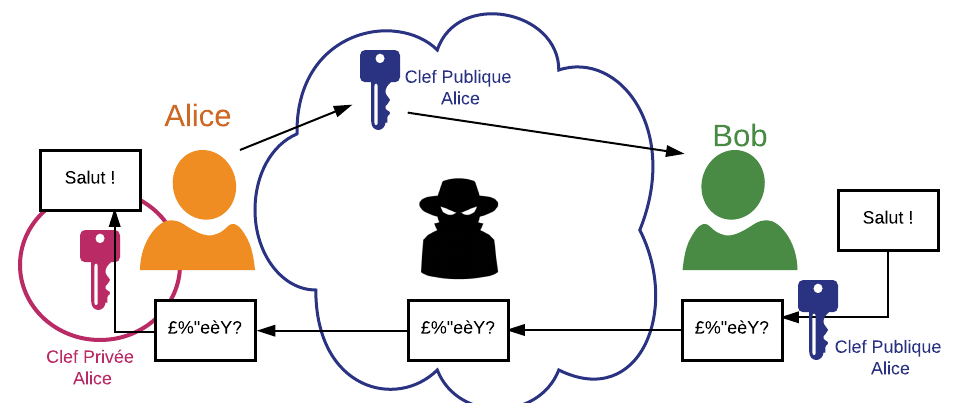
\includegraphics[keepaspectratio, scale=0.35]{figures/chiffrement.png}
	\pause
	\begin{itemize}
	\item L'espion ne peut pas lire !
	\end{itemize}
\end{frame}

\subsection{Signature}
\begin{frame}{La signature}
	\begin{itemize}
	\item \textbf{Signe} avec clef \textbf{privée} | \textbf{Vérifie} clef \textbf{publique}
	\end{itemize}
	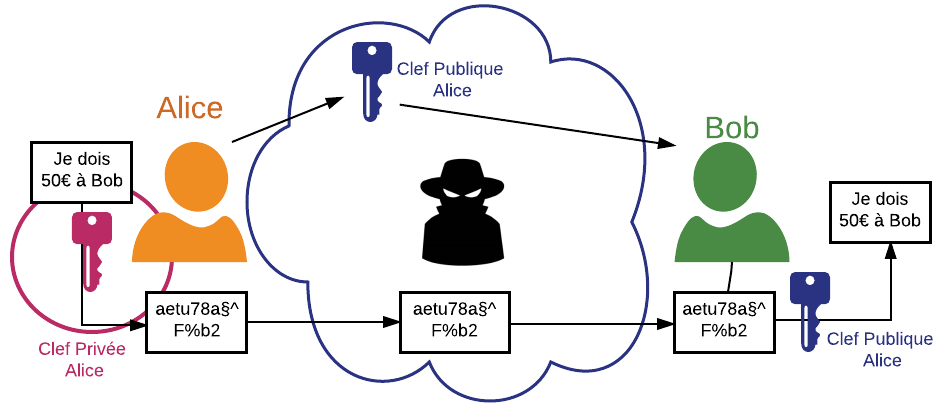
\includegraphics[keepaspectratio, scale=0.36]{figures/signature1.png}
\end{frame}

\begin{frame}{La signature}
	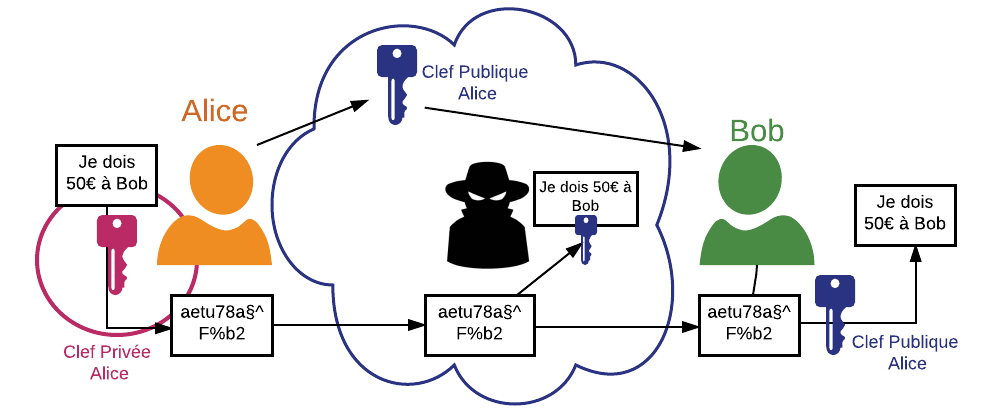
\includegraphics[keepaspectratio, scale=0.36]{figures/signature2.png}
	\begin{itemize}
		\item Tout le monde peut vérifier !
		\item L'espion ne peut pas imiter la signature d'Alice !
	\end{itemize}
\end{frame}
\subsection{PGP, OpenPGP, GPG ??}
\begin{frame}{PGP, OpenPGP, GPG, ... ???}
	\begin{itemize}
	\item PGP : Pretty Good Privacy
	\item OpenPGP : Equivalent libre de PGP \\ Standard qui définit le format de clefs, de messages, etc.
	\item GPG (GnuPG) : Gnu Privacy Guard, implémentation logicielle\\ ~ \\ ~ \\
	\item et BGP ? : Border Gateway Protocol  --> Rien à voir
	\end{itemize}
\end{frame}



\section{Pratique}
\subsection{Création paire de clefs}
\begin{frame}
\frametitle{Création paire de clefs}
\vspace*{-0.5cm}
Outil GnuPG (\textbf{gpg2}) \hspace*{2.5cm} ({\color{gray}Interface graphique : seahorse})\\~\\
\textbf{gpg2 -~-gen-key}
\begin{itemize}
\item RSA 
\item 4096bits
\item expiration
\item infos persos
\item passphrase
\end{itemize}
\end{frame}

\begin{frame}
\frametitle{Cheatsheet}
    \begin{tabular}{ | l | l |}
    \hline
    \multicolumn{2}{|c|}{Cheatsheet} \\ \hline
    gpg2 -~-list-keys & Liste toutes les clefs sur la machine \\ \hline
    gpg2 -~-keyserver <serveur>  & Exporte une clef publique \\  
    -~-send-key <id> & sur un serveur de clef\\ \hline
    gpg2 -~-keyserver <serveur> & Cherche une clef publique \\
    -~-search-keys <id> & sur le serveur \\ \hline
    gpg2 -~-keyserver <serveur> & Importe une clef publique \\
     -~-recv-keys <id> &  depuis le serveur\\ \hline 
    gpg2 -~-delete-keys <id> &  Supprime une clef publique du trousseau\\  \hline
    gpg2 -~-gen-revoke & Révoque votre \textbf{propre clef publique}\\
     <votre\_email> & \\
     \hline
    \end{tabular}  
    ~\\  
    Exemple de serveur : pgp.mit.edu  : \\
    \textbf{gpg -~-keyserver hkp://pgp.mit.edu \\-~-search-keys "Nom de quelqu'un"}
\end{frame}
\subsection{Enigmail}


\begin{frame}
\frametitle{Enigmail}
    Voir démo\\
    \begin{itemize}
    \item Suivre le Setup Wizard en mode avancé 
    \item Choisir "j'ai déjà des clefs"
    \item Si les clefs ne sont pas repérés :
    	\begin{itemize}
    	\item \textbf{cd ; cd .gnupg/}
    	\item \textbf{gpg2 -~-export votre\_mail >  publickey.asc}
    	\item \textbf{gpg2 -~-export-secret-key votre\_mail >  privatekey.asc}
    	\item Dans Thunderbird, choisir publickey.asc et privatekey.asc créés dans le dossier ~ $_{\widetilde{~}}$.gnupg
    	\item Une fois que le setup wizard est terminé : \textbf{rm privatekey.asc} (pour ne pas laisser trainer la clef dans le dossier...)
    	\end{itemize}
   \item Lors de l'écriture d'un mail, choisir "chiffrer" et/ou "signer" dans le menu Enigmail.
  	
    \end{itemize}
    Aide : http://enigmail.wiki/ 
 \end{frame}
 
\subsection{OpenKeyChain (Android)}

\begin{frame}
\frametitle{OpenKeyChain (Android)}
\begin{itemize}
    \item Créer une paire de clefs personnelle 
    \item Gérer les clefs publiques de vos amis 
    \begin{itemize}
    \item Ajout facile (QR code !, et depuis serveur) 
    \end{itemize}
    \item Chiffre/déchiffrer des documents 
    \item Faire des sauvegardes/imports
    \item  Compatible avec plein d'applis : \\
    K9-Mail, Conversations (chat), Password Store, etc. :-)
  \end{itemize}
\end{frame}


\begin{frame}
\frametitle{OpenKeyChain}
\centering
    	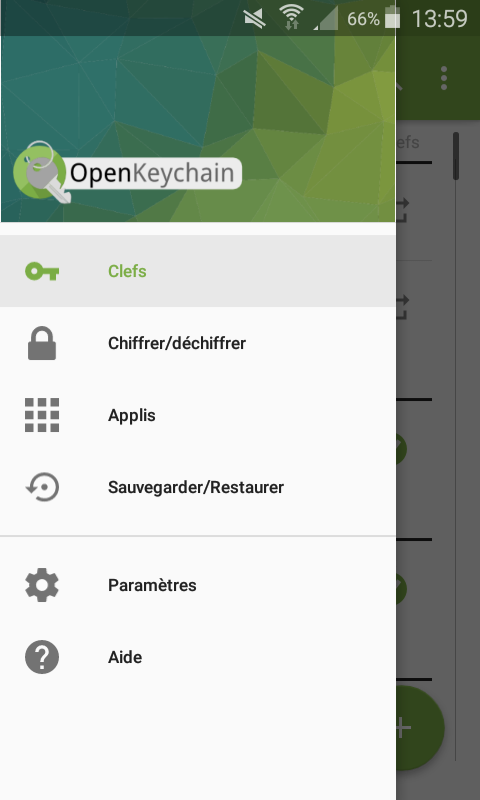
\includegraphics[keepaspectratio, scale=0.25]{figures/okc.png}
\end{frame}


\subsection{K9-Mail (Android)}


\begin{frame}
\frametitle{K9-Mail }
\centering
    	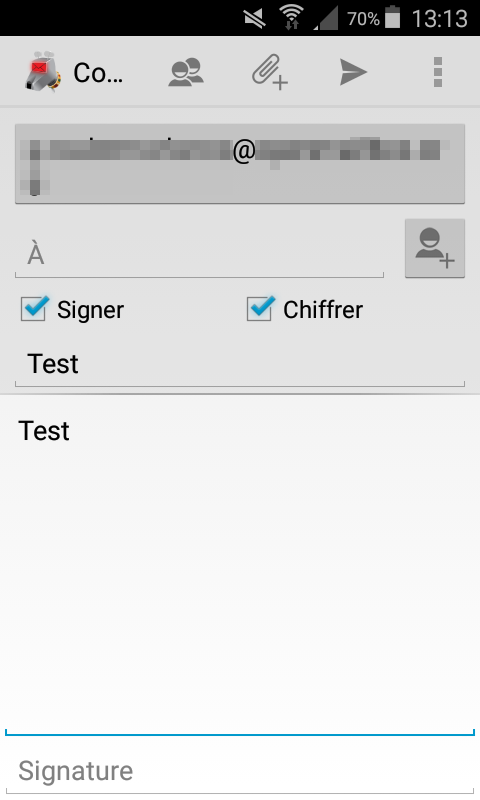
\includegraphics[keepaspectratio, scale=0.25]{figures/K90.png}
\end{frame}



\begin{frame}
\frametitle{K9-Mail}
\begin{minipage}{0.4\textwidth}
\centering
    	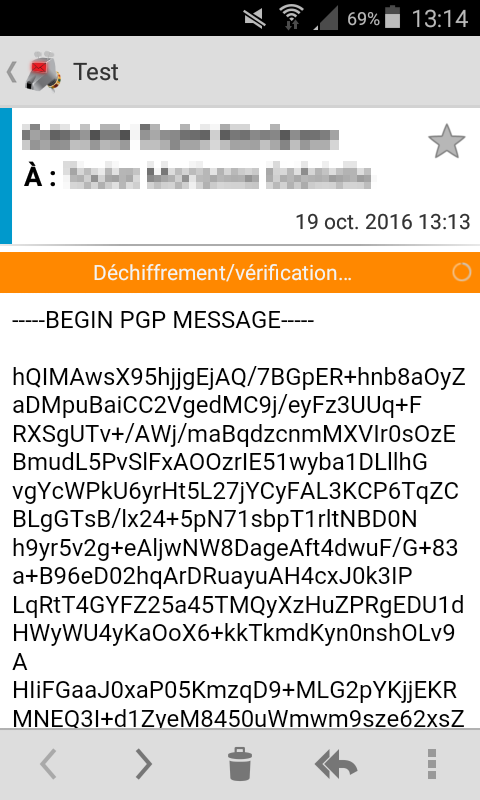
\includegraphics[keepaspectratio, scale=0.25]{figures/K91.png}
    	\end{minipage}
\begin{minipage}{0.4\textwidth}
\centering
    	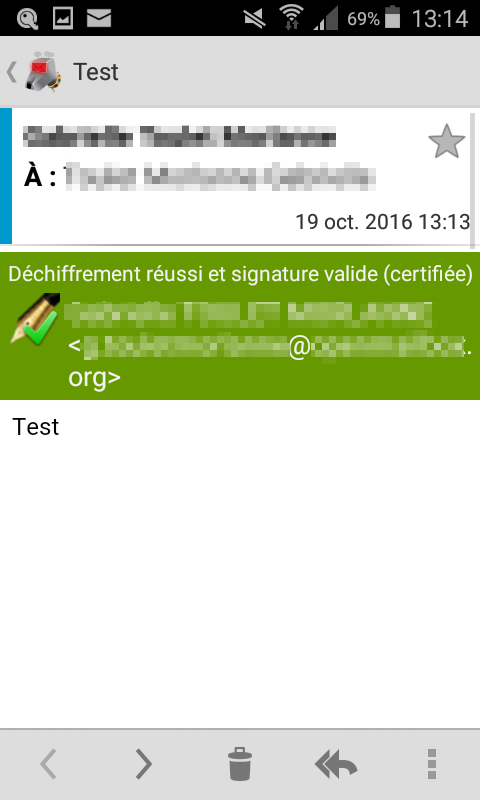
\includegraphics[keepaspectratio, scale=0.25]{figures/K92.png}
\end{minipage}
\end{frame}


\end{document}
